\section{Foundation Heat Transfer Calculations using BASESIMP}\label{foundation-heat-transfer-calculations-using-basesimp}

BASESIMP (Beausoleil-Morrison and Mitalas, 1997) is a foundation heat transfer model developed by the Canadian government and implemented into their residential simulation packages, i.e. HOT2000 and HOT3000, to assess the thermal performance of small Canadian residential buildings.  As such, it can model most of the foundations encountered in Canadian houses.

Its calculation method is based on regressions, making the model computationally fast.  The coefficients of these regressions were developed from a large number of simulations performed using another foundation heat transfer model named BASECALC (Beausoleil-Morrison et al., 1995).  BASECALC uses a combination of 2-D finite-elements simulations and corner correction factors to obtain quasi-3D solutions for heat transfer around foundations.


\subsubsection{Approach}\label{approach-basesimp}

BASECALC and BASESIMP break up heat transfer from a foundation in three parts: the above grade heat losses ($q_{ag}$), the average (or constant) below grade heat transfer ($q_{bg,avg}$), and the harmonic (or variable) below grade losses ($q_{bg,var}$).  This results in an equation of the type:
\begin{equation} \label{eq:BASESIMPEquation}
    q_{fnd} = q_{ag} + q_{bg,avg}  + q_{bg,var}
\end{equation}
Where:
\begin{equation} \label{eq:AGLossesEquation}
    q_{ag} = S_{ag} \: \left( \overline{T}_{zone} - T_{amb} \right)
\end{equation}
\begin{equation} \label{eq:BGAvgLossesEquation}
    q_{bg,avg} = S_{bg, avg} \: \left( \overline{T}_{zone} - T_{g,avg} \right)
\end{equation}
And:
\begin{equation} \label{eq:BGVarLossesEquation}
    q_{bg,var} = S_{bg, var} \: T_{g,amp} \: sin \left( \frac{2 \: \pi}{8760} \: t - \frac{\pi}{2} - T_{g,ps} - Phase \right)
\end{equation}
Where:
\begin{itemize}
    \item $t$ is the time in hours.
    \item $S_{ag}$, $S_{bg, avg}$, and $S_{bg, var}$ are heat transfer coefficients (W/K).
    \item $\overline{T}_{zone}$ and $T_{amb}$ are the foundation zone and ambient (outdoor) temperatures ($^{\circ}C$).
    \item $T_{g,avg}$ and $T_{g,amp}$ are the average ground surface temperature and the amplitude of its annual variation ($^{\circ}C$).
    \item $T_{g,ps}$ is a phase lag representing the period between the first of January and the time when the coldest ground surface temperature is observed (rad).
    \item $Phase$ is a phase lag representing the thermal response of the foundation/soil system (rad).
\end{itemize}

At the beginning of the simulation, BASESIMP evaluates the values of $S_{ag}$, $S_{bg,avg}$, $S_{bg,var}$, and {$Phase$}. The soil temperature parameters ($T_{g,avg}$, $T_{g,amp}$, and $T_{g,ps}$) are provided by the user as inputs.  Using the time, the zone temperature, and the ambient temperature to solve Equation \ref{eq:BASESIMPEquation} to assess the foundation heat losses at every iteration of a simulation is simple and quick.

38 coefficients and 19 corner factors are required to evaluate $S_{ag}$, $S_{bg,avg}$, $S_{bg,var}$, and $Phase$: as a function of foundation type, material, insulation performance and placement, dimensions, soil properties, and water table location.  These coefficient depend on the combination of foundation type, material, and insulation placement: i.e. the configuration of the foundation.  The current version of BASESIMP can model 117 configurations (67 basements and 50 slabs).  These configurations are listed by Pinel (2016) among others.  Users can also calculate the coefficients ($S_{ag}$, $S_{bg,avg}$, $S_{bg,var}$, and $Phase$) with BASECALC and enter them directly when the studied configuration is not in the database.

\subsubsection{Parameters}\label{parameters-basesimp}

As previously explained, BASESIMP models can be defined with two methods, specified with a ``Model Type" parameter: the user can supply the calculated BASECALC coefficients or a description of the foundation.  Seven parameters are read for all foundations: the foundation name, the name of the affected building zone, the model type, the fraction of the losses calculated by BASESIMP to be extracted from the zone, and the three parameters describing the soil surface temperature ($T_{g,avg}$, $T_{g,amp}$, and $T_{g,ps}$).  If the model is of the type ``BASECALC coefficients", the four BASECALC coefficients ($S_{ag}$, $S_{bg, avg}$, $S_{bg, var}$, and $Phase$) are read.  If it is of type ``Foundation description" then a variable number of parameters may be read depending on the foundation configuration: w/wo insulation, w/wo overlap, etc.

Table \ref{table:BSFoundationParameters} presents the requirements for both types of models.  An ``x" signifies that a value is required in the field associated with the parameter in the BASESIMP object representing the modelled foundation.

\begin{longtable}{lcc}
\hline
\textbf{Parameter }             & \textbf{Foundation description}   & \textbf{BASECALC coef.}     \\
\hline
\hline
Name                            & x                                 & x                         \\
Zone name                       & x                                 & x                         \\
Model Type                      & x                                 & x                         \\
Foundation type                 & x                                 &                           \\
Foundation material             & x                                 &                           \\
                                & Must be concrete for slabs        &                           \\
BSConfig(Conc B)                & If concrete basement              &                           \\
BSConfig(Wood B)                & If wood basement                  &                           \\
BSConfig(Wood\&Conc B)          & If wood\&concrete basement     &                           \\
BSConfig(Concrete S)            & If slab-in-grade                  &                           \\
BASESIMP Fraction               & x                                 & x                         \\
Foundation height               & x                                 &                           \\
Foundation depth                & x                                 &                           \\
Foundation length               & x                                 &                           \\
Foundation width                & x                                 &                           \\
Wall insulation overlap         & If overlap in config              &                           \\
Insulation resistance           & If insulation in config           &                           \\
Soil thermal conductivity       & x                                 &                           \\
Water table depth               & x                                 &                           \\
AG losses coef                  &                                   & x                         \\
BGavg coef                      &                                   & x                         \\
BGvar coef                      &                                   & x                         \\
Thermal response ($Phase$)      &                                   & x                         \\
Average ground temperature      & x                                 & x                         \\
Temperature variation amplitude & x                                 & x                         \\
Phase lag ($T_{g,ps}$)          & x                                 & x                         \\
\hline
\caption{Required parameters for the two model types} \label{table:BSFoundationParameters}
\end{longtable}


\subsubsection{Boundary Conditions}\label{boundary-conditions-basesimp}

Since BASESIMP is based on BASECALC simulations, the same boundary conditions apply.  The following boundary conditions are assumed when running a BASECALC simulation:
\begin{itemize}
    \item Ground surface: No weather is considered at the surface.  The user enters three parameters destined to model the ground surface temperature as a sinusoidal function (Equation \ref{eq:BGVarLossesEquation}).
    \item Bottom of the domain: A constant temperature water table is assumed to be located at the bottom of the domain: at a depth indicated by the user. This temperature is equal to the average ground surface temperature.
    \item Far field: An adiabatic plane is inserted at a distance from the basement representing the mid-point to the neighbouring house.
    \item Foundation zone:  The exact temperature of the indoor zone is not really relevant since BASECALC computes heat losses as a function of difference between this temperature and the ambient temperature ($T_{zone}-T_{amb}$) as well as with the soil surface temperature ($T_{zone}-T_{soil}$).  A constant conductance coefficient, accounting for convection and long wave radiation, is assumed between the zone air node (temperature) and the foundations.
\end{itemize}

\subsubsection{Other Assumptions}\label{assumptions-basesimp}

In the conception of the algorithm, some assumptions were made regarding construction of the foundation and soil properties.  These constitute proper approximations for most foundations encountered in the practice.  For foundations that deviate considerably from these assumption, a more flexible evaluation method may be more appropriate.  It is assumed that:
\begin{itemize}
    \item The density and specific heat of the soil are $1490 \: kg/m^3$ and $1800 \: J/kgK$ respectively.
    \item The foundations' walls and floor/slab all have the same thickness: concrete basements have $200 \: mm$ walls and $100 \: mm$ floors while wood basements have $50 \: mm$ walls and $100 \: mm$ floors.
        For soils/walls/slabs deviating substantially from these values, the algorithm can therefore miss short term thermal mass effects: rapid temperature fluctuations for example.  This should not affect monthly energy balances, though, as those are nearly steady state.
    \item For configurations having combination insulation (e.g. interior of walls + slab, interior + exterior of walls, etc.), the same level of insulation is present everywhere.
        Sensitivity runs showed that, as long as the resistance of interior and exterior insulation are within 65 \% of each other, setting the exterior insulation identical to the interior one makes less than a 5 \% difference in the results. No mention of such a sensitivity study for walls and floor combinations were found during this review though.
\end{itemize}

\subsubsection{Limits}\label{limits-basesimp}

BASESIMP includes several limits.  The regressions were conceived  by varying parameters within ranges extending from lower to higher limits.  It is not recommended to use them outside of these ranges as using extrapolations instead of interpolations is always risky.  These limits include:
\begin{flushleft}
\begin{itemize}
    \item the width of foundations must be between $5$ and $12 \: m$ and be smaller than the length: $5 \leq width \leq 12$ and $width \leq length$;
    \item the height of basements must be between $1.0$ and $2.5 \: m$: $1.0 \leq height \leq 2.5$;
    \item the depth (below ground) of basements must be between $0.65$ and $2.4 \: m$: $0.65 \leq depth \leq 2.4$;
    \item the above grade section of the basement must exceed $0.1 \: m$: $height-depth \geq 0.1$;
    \item the soil thermal conductivity must vary between $0.85$ and $1.9 \: W/mK$: $0.85 \leq soilk \leq 1.9$
    \item the insulation resistance must vary between $1.5$ and $9.0 \: m^2K/W$: $1.5 \leq rsi \leq 9.0$;
    \item the overlap between interior and exterior wall insulation must vary between $0$ and $2.4 \: m$ and be smaller than the basement depth: $0 \leq overlap \leq 2.4$ and $overlap \leq depth$;
    \item the water table must be located at a depth varying between $5$ and $15 \: m$: $5 \leq wtable \leq 15$;
\end{itemize}
\end{flushleft}

To circumvent lower end of the $6^{th}$ limit from this list, i.e. the lower limit on insulation performance (RSI $\geq$ 1.5), the implementations of the model include an interpolation algorithm which is applied whenever the specified insulation performance is between 0 and 1.5 RSI.  The technique consists of evaluating the coefficients for the foundation with 1.5 RSI insulation and with no insulation.  From there, an ``exponential interpolation" technique is applied to evaluate the coefficients for the specified insulation performance ($RSI_{ins}$).


\subsubsection{Implementation and use in EnergyPlus}\label{beaseSimp-Eplus}

Figure \ref{fig:BASESIMPCoupling} illustrates the coupling of a BASESIMP model with a whole building in EnergyPlus.  Since BASESIMP evaluates the heat losses from the entire foundation, there is no point in modelling foundation walls and floors.  Heat losses are passed to the affected zone as negative internal gains.
\begin{figure}[htbp]
\centering
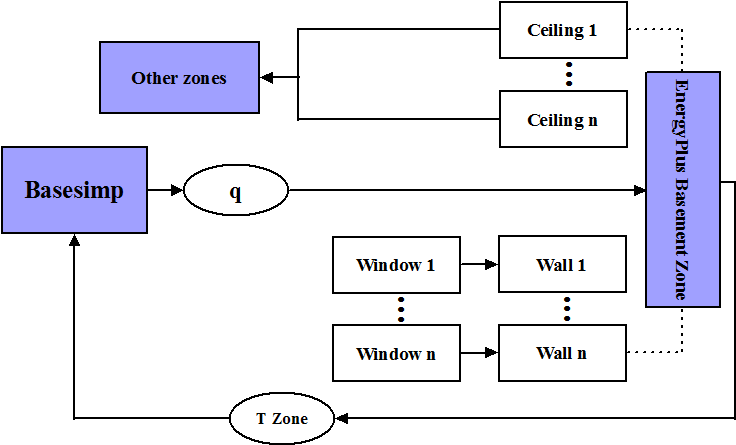
\includegraphics{media/image8010.png}
\caption{BASESIMP foundation coupling with whole building.} \label{fig:BASESIMPCoupling}
\end{figure}

The only surfaces that need to be modelled in the EnergyPlus model are those that provide coupling with other zones (the ceilings in Figure \ref{fig:BASESIMPCoupling}) of the building and those that are used to support windows and doors (the walls in Figure \ref{fig:BASESIMPCoupling}).  However, since not modelling these surfaces results in a zone that is not enclosed, the correct volume should be specified in the corresponding Zone object.

So setting up a BASESIMP model requires:
\begin{enumerate}
    \item Setting up a Zone object, representing a basement zone or the zone above a slab-in-grade foundation.  Making sure to specify the correct floor area, height, and volume in this object.
    \item Specifying only the surfaces that are not part of the foundation in that zone.  Note that EnergyPlus requires at least one surface per zone.
    \item Creating a BASESIMP object and specifying the created zone in this object.
\end{enumerate}

\subsubsection{Addition of windows to foundation}\label{beaseSimp-windows}

The BASESIMP regressions were developed for foundations that do not include windows.  Since windows require walls for support, walls must be modelled.  In order not to add too much heat exchange surface to the basement zone, these walls should be just large enough to accommodate the modelled windows. EnergyPlus does not accept windows modelled on adiabatic walls so limiting the walls dimensions is the only way to limit the increase in heat exchange area.

The windows should be added on these support walls.  However, the area occupied by these windows is modelled as a foundation wall by BASESIMP.  To compensate, it is recommended to deduct the thermal conductance (U = 1/R) of the foundation wall from that of the modelled window.  For a window with a thermal conductance $U_{window}$ on a foundation wall with a conductance $U_{wall}$, this yields for the modelled window conductance $U_{window,mod}$:
\begin{equation}
U_{window,mod} = U_{window} - U_{wall}
\end{equation}


References:

Beausoleil-Morrison, I. \& Mitalas, G. 1997. `BASESIMP: A residential foundation heat loss algorithm for incorporating into whole-building energy analysis programs` Building Simulation 97, International Building Performance Simulation Association, Prague, Czech Republic, pp. 1-8.

Beausoleil-Morrison, I., Mitalas, G. \& McLarnon, C. 1995. `BASECALC: new software for modelling basement and slab-on-grade heat losses`, Building Simulation 95, International Building Performance Simulation Association, Madison, U.S., pp. 698-700.

Pinel,P. 2016. Addition of the BASESIMP Foundation Model to EnergyPlus, Report for CanmetENERGY, Natural Resources Canada, Ottawa, Canada.
